\section{Introduction}

\subsection{Background}
Authentication is the process of confirming the validity of a claimed identity seeking access to a system or resource. Over decades, authentication mechanisms have evolved from basic password systems in the 1960s to advanced methods such as multifactor authentication by the late 2010s, driven by a persistent commitment to combat evolving security risks while enhancing user convenience\cite{ref1}. Various methods such as password-based authentication, certificate-based authentication, one-time passwords, multifactor authentication, and biometric authentication are employed\cite{ref2}.

Biometric authentication, which involves analyzing unique physical characteristics, is often considered more secure than traditional authentication methods due to the difficulty in duplicating biometric traits. This encompasses technologies such as facial recognition, fingerprint recognition, eye recognition, and voice recognition\cite{ref3}.
However, despite the enhanced security of biometric authentication, it is not immune to exploitation. For instance, fingerprints left on surfaces can be copied, or hackers may obtain images of individuals online to deceive authentication systems.
Choosing the right authentication mechanism requires careful consideration of various factors including the necessary security level, ease of use for users, cost implications for setup and ongoing upkeep, as well as the unique risks and vulnerabilities pertinent to the system or data in question. Typically, the requisite level of security steers the selection process; for example, platforms managing sensitive personal information might mandate the use of robust authentication methods, such as biometric verification. The inherent challenge in deploying such secure systems lies in achieving a delicate equilibrium between high security measures and user convenience. The goal is to create an authentication process that is both seamless and efficient, ensuring that access is granted swiftly and accurately to the rightful user without necessitating multiple attempts, thus maintaining a user-friendly experience while upholding the highest security standards.

While advanced biometric systems typically rely on externally visible physical attributes, finger-vein authentication focuses on internal anatomical features, adding a unique layer of security, as they are less prone to replication or theft compared to external characteristics. Nevertheless, it is important to note that finger-vein authentication does not completely eliminate challenges. Despite its emphasis on internal features, attackers can exploit inherent structures in finger veins, such as common patterns among individuals and predictability in acquired data, which poses risks to the authentication process.\\

In light of these considerations, this project is dedicated to authentication using finger-vein features.
This involves utilizing a specialized scanner equipped with two infrared cameras to capture finger veins from different angles.
The registration process involves capturing an image, termed the model image, while the authentication process involves capturing another image, known as the probe image. These images undergo processing through a pipeline designed to extract and align the finger-vein patterns.
The pipeline outputs a feature vector, which is essentially a bitstring, where 0's represent where there are no finger veins, and 1's show where veins are present.
Following this process, the system evaluates whether the feature vector extracted from the probe image sufficiently matches the feature vector of the model image associated with the individual attempting authentication.

\subsection{Extraction Pipeline}\label{sec:extraction-pipeline}

This project extends the work on optimizing a finger-vein recognition pipeline that has demonstrated the lowest \hyperref[def:EER]{Equal Error Rate (EER)} by incorporating a novel hashing step to process the output of the pipeline. The purpose of integrating \hyperref[def:Hash_Function]{Hash Functions} within this context is multifold, but before delving into hash functions, which are central to our project, it's essential to outline the foundation upon which we have built our advancements. This initial context will provide a clearer understanding of the starting point from which our developments began.\\

Simon Sommerhalder and Burcu Yildiz have both made significant contributions to the system. Simon introduced an innovative approach to the alignment of freshly captured images (probe images) with those stored in the system (model images), ensuring the hashing process (following the alignment of the finger) is based on the unique finger-vein pattern rather than how the finger is positioned on the scanner.

Simon has developped a pipeline (see Figure~\ref{pipeline_simon}) to align finger-vein images, enhancing security by eliminating the need to compare the model and probe images side by side. He organized the pipeline into six clear steps:

\begin{enumerate}
    \item \textbf{Masking}: The first step of the pipeline isolates the finger area in the image. This involves creating a mask that outlines the finger, ensuring that subsequent processing focuses solely on the relevant part of the image.

    \item \textbf{Prealignment}: This step involves adjusting the position and orientation of the finger within the image before extracting vein patterns. It's aimed at roughly aligning the image based on the finger's outline, helping to standardize the position of the finger across different scans.

    \item \textbf{Histogram equalization}: To ensure the images have consistent lighting and contrast, this step adjusts the brightness levels. This makes the vein patterns more distinct and comparable across different images.

    \item \textbf{Feature extraction}: Here, the actual vein patterns are identified and extracted from the image. The process converts the visual image into a digital format that represents the presence or absence of veins at specific locations.

    \item \textbf{Postalignment}: After extracting the vein patterns, this step fine-tunes the alignment of the image. It's based on the vein patterns themselves, ensuring that the comparison between model and probe images is as accurate as possible.

    \item \textbf{Distance Calculation}: The final step involves comparing the feature vector of the probe image with that of the model image. This is done using a specific metric to quantify the similarity between the two, ultimately determining if they match closely enough for authentication to succeed.
\end{enumerate} 

\begin{figure}[!h]
    \centering
    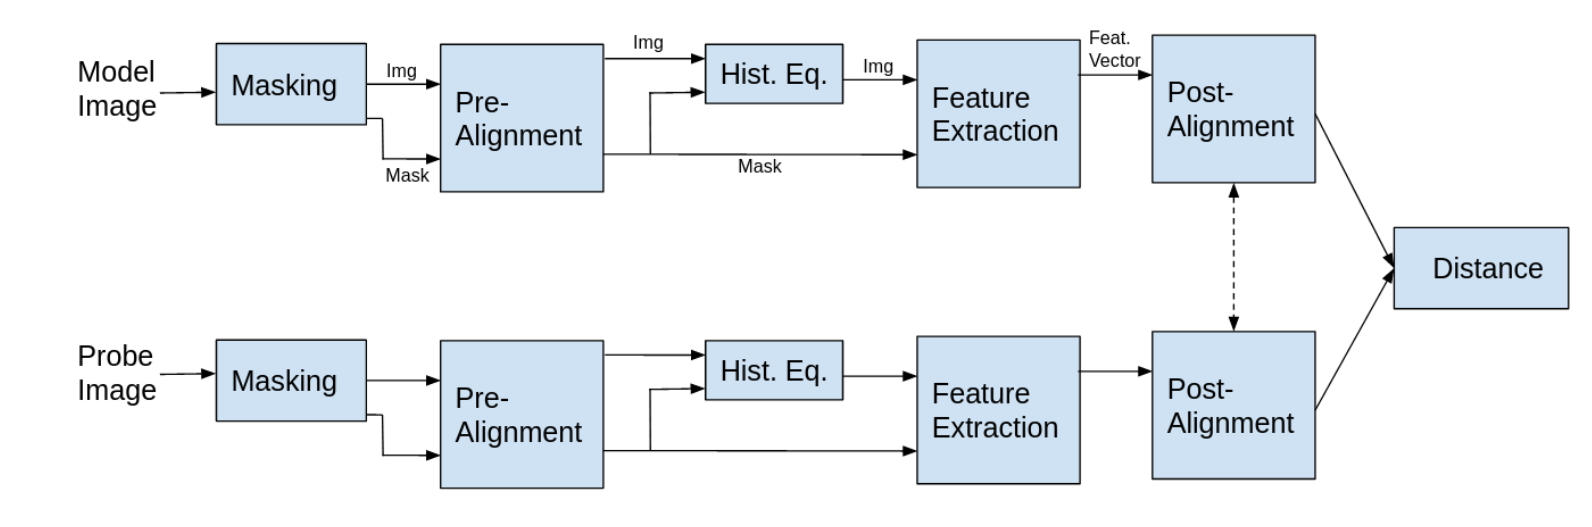
\includegraphics[width=1\linewidth]{latex-img/pipeline_simon.png}
    \caption{Simon's Extraction Pipeline. Compares a single probe image to a model image}
    \label{pipeline_simon}
\end{figure}

Burcu's work on the finger vein authentication project built upon Simon's foundational pipeline, focusing on refining image processing for vein extraction and evaluating different distance calculation methods for authentication. She optimized preprocessing steps, investigated masking and prealignment issues, and tackled reference selection to enhance matching accuracy. A significant part of her contributions involved exploring fuzzy extractors \hyperref[def:Fuzzy_Extractors]{Fuzzy Extractors} to bolster security, conducting a thorough analysis of the dataset to identify and address challenges, and proposing solutions to improve the system's reliability and efficiency.\\

Simon and Burcu explored a variety of function combinations at different stages of the authentication pipeline, aiming to pinpoint the configuration that yields the most favorable outcomes. They utilized the Equal Error Rate (EER) as a benchmark to measure the pipeline's efficacy, focusing on achieving a balance between security and accessibility. This metric, representing the point where the rate of false acceptances (impostor incorrectly granted access) matches the rate of false rejections (legitimate user incorrectly denied), serves as an indicator of the system's reliability and accuracy. The configuration that demonstrated superior performance, leading to the lowest EER and thereby optimizing the process of analyzing and processing images, is showcased in the subsequent figure.

\begin{table}[H]
    \centering
    \caption{EER values for the best pipeline: Edge masking, translation pre-alignment, no pre-processing, no post-
    processing, Miura matching as the post-alignment}
    \begin{tabular}{lc}
    \toprule
    Camera & EER \\
    \midrule
    Camera 1 & 0.041 \\
    Camera 2 & 0.029 \\
    Sum of cameras & 0.030 \\
    \bottomrule
    \end{tabular}
    \label{tab:eervalues_best}
\end{table}

\subsection{Project Overview}

In the progression of our project, building upon the work of Simon and Burcu, we aim to address the inherent variability in biometric data, particularly with finger vein patterns, by considering hash functions. The final objective of the system is to add a hashing step at the end of our established pipeline, prior to the post-alignment phase. The integration of this step serves to enhance security and overall functionality by allowing us to store a hash of each biometric image X in our database, instead of the raw biometric data. Upon receiving a new image Y, we compute hashes for all potential translations of Y, comparing these with the hash of X. Unfortunately, this process is computationally expensive because it requires computing the hash for every possible translation of the image. The purpose of employing a hashing process in this system is multifold:

\begin{itemize}
    \item \textbf{Security}: Hash values can be stored instead of raw biometric data. In the event of a database breach, attackers would find it significantly more challenging to reconstruct the original biometric information from the hashed values due to the one-way nature of hash functions.

    \item \textbf{Consistency}: By focusing on the unique patterns of the biometric trait (like finger-vein patterns) and standardizing how this data is processed and hashed, the system aims to produce consistent hash values for the same individual across different scanning sessions. This is crucial for reliable authentication, ensuring that minor variations in finger placement do not affect the system's ability to recognize the user.

    \item \textbf{Performance}: Hashing biometric data into a compact, fixed-size format facilitates quicker comparison and verification processes. It's more efficient to compare hash values than to perform complex pattern recognition operations on raw biometric images.
\end{itemize}

Traditional hash functions, while pivotal in various data security contexts, generate a unique output for each unique input. This one-to-one mapping means even minor variations in the input — common in biometric data due to natural changes in biological traits or differences in scanning conditions — result in completely different hashes. This sensitivity to input variability poses a challenge in biometric authentication systems, where the goal is to accurately recognize and authenticate an individual despite these natural variations.

Fuzzy hashing stands as a sophisticated solution to this challenge. Unlike traditional hash functions, fuzzy hashing is designed to produce consistent cryptographic keys for inputs that are similar, but not identical. This is particularly advantageous in biometric authentication systems, where it's essential to recognize the same biometric trait across different instances, despite slight variations. The "fuzziness" of this approach allows the system to map these similar inputs to the same or closely related hash values, thereby ensuring that legitimate users are not incorrectly denied access due to minor discrepancies in their biometric data.
Furthermore, the application of fuzzy hashing in our pipeline is instrumental in protecting user privacy. Since the hashed values, rather than raw biometric data, are stored and used for authentication, users' biometric information is safeguarded against potential breaches. Even if hashed values were accessed without authorization, the complexity of fuzzy hashing algorithms makes it extremely challenging to reverse-engineer the original biometric data.\\

The process of our fuzzy hashing algorithm, that we will detail in Section~\ref{sec:Fuzzy Hashing}  begins with a biometric capture, a finger image, which goes through the already developped pipeline~\ref{pipeline_simon} to extract a bitstring. This bitstring undergoes a pre-hashing process, where a subset of significant bits (denoted as vein pixels) is selected based on a permutation keyed by a secure key, resulting in a tuple that significantly reduces the data's dimensionality while preserving its distinguishing features.

Upon generating the fuzzy hash, the next step involves further compressing this hash to prepare it for storage. This compression is achieved through a function, postHash, which maps the tuple to a bitstring of a defined length. The output, essentially a compressed fuzzy hash, exhibits nearly uniform distribution when both the input data and the key are random, enhancing security and storage efficiency.

To further bolster the security of the stored biometric data, this system incorporates \hyperref[def:Fuzzy_Extractors]{Fuzzy Extractors}. The fuzzy extractor framework ensures that even if the stored data is compromised, reconstructing the original biometric data or compromising individual privacy remains computationally infeasible. This is accomplished by generating a secure, random key from the biometric input using a generation process (Gen) and allowing for the reliable reproduction of this key from an approximation of the original input using a reproduction process (Rep), without directly storing the biometric data itself.

In essence, we aim to store the output of the fuzzy extractor, which includes the reproducible cryptographic key and the helper data, instead of the raw biometric data or its direct hash. This method ensures that the stored biometric data is not only compact and efficiently stored but also securely obfuscated, requiring the correct biometric input for any form of decryption or matching to occur.



\section{Fuzzy Hashing}
\label{sec:Fuzzy Hashing}
Fuzzy hashing, as opposed to traditional hashing, produces consistent cryptographic keys for similar but not identical inputs, enabling recognition of the same biometric trait across different instances despite slight variations. This approach ensures legitimate users are not incorrectly denied access due to minor discrepancies and protects user privacy by storing and using hashed values instead of raw biometric data, making it difficult to reverse-engineer the original data even if unauthorized access occurs. 
This section will discuss how we implemented the fuzzy hashing algorithm, its corresponding mathematical aspects and some experiments.

\subsection{PreHashing Algorithm}

The \textit{PreHash} algorithm is the first step in the fuzzy hashing process, designed to manipulate biometric templates extracted from finger vein patterns. It operates on a bitstring \(X\), representing the presence (1) or absence (0) of vein pixels across \(n\) pixels, where \(n=96'500\).

Algorithm Inputs and Outputs:
\begin{enumerate}
    \item \textbf{Inputs}: The algorithm takes three main inputs:
    \begin{itemize}
        \item \textbf{A parameter m}: the number of indices to find
        \item \textbf{A bitstring X}: the feature-extracted vein patterns of a biometric capture
        \item \textbf{A key}: used to initialize a Pseudorandom Number Generator (PRNG)
    \end{itemize}
    \item \textbf{Output}: The algorithm outputs a tuple \((i_1,...,i_m)\) consisting of the \(m\) smallest indices \(i_j\)​ such that \(1 \leq i_1<...<i_m\)​ and the pixel at \(PRNGkey(i_j)\) in \(X\) is identified as a vein pixel. 
\end{enumerate}

Detailed Process of \textit{PreHash}:
\begin{itemize}
    \item \textbf{Initiallization}: Utilizing the provided key, the algorithm initializes a PRNG. This PRNG is based on the \hyperref[def:AES CTR mode]{Advanced Encryption Standard (AES) in Counter (CTR) mode}, ensuring the generation of uniform and independent pseudorandom sequences.

    \item \textbf{Nonce Generation}: A nonce in CTR mode encryption is initialized to zero to maintain simplicity and security. We opted against using a keyed hash function to generate the nonce, as it would tie the nonce to the secret key. Such a dependency would mean that both the nonce and the Pseudo-Random Number Generator (PRNG) would rely on the same key, creating a security risk by concentrating security on a single element. To avoid this, we keep the generation of the nonce separate from the key.

    \item \textbf{Pseudorandom Sequence Generation}: Upon receiving the parameters—key, nonce, and counter—the PRNG operates in CTR mode to generate a 128-bit pseudo-random number. As depicted in Figure~\ref{ctr encryption}, this process involves encrypting the nonce combined with the counter using the key. The output from this block cipher encryption phase is then XORed with a vector consisting of zero bits. Since we require 17 bits for our application, the block cipher's output is XORed with a bitstring of 3 bytes to achieve the necessary length. To ensure the output meets the project's specific requirements, it is then masked to retain only the top 17 bits. This adjustment is essential as it aims to ensure that pseudo-random numbers are generated within a suitable range form image size, specifically \(96'500\) pixels, which requires \(17\) bits for representation\footnote{\(\lceil \log_2(96'500) \rceil = 17\)}. The predictability of this sequence is entirely dictated by the chosen key. In essence, employing the same key will consistently yield an identical nonce and hence an identical sequence of numbers.

    \begin{figure}[!h]
        \centering
        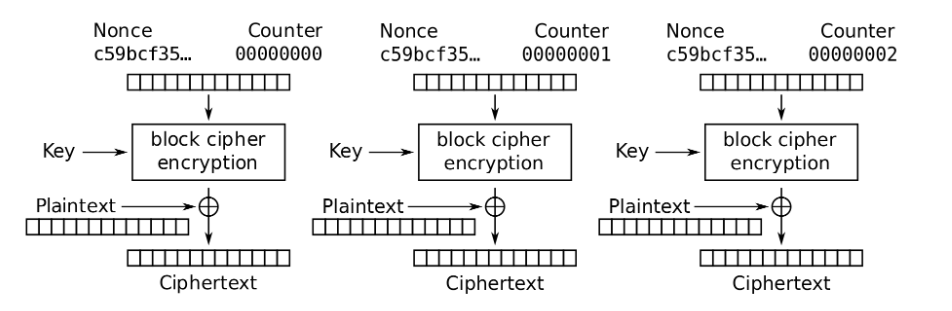
\includegraphics[width=1\linewidth]{latex-img/CTR_encryption.png}
        \caption{Counter (CTR) mode encryption}
        \label{ctr encryption}
    \end{figure}

    \item \textbf{Selection of Indices}: The algorithm iterates through the generated pseudorandom sequence, selecting the first \(m\) indices corresponding to vein pixels in the biometric template \(X\). This selection process involves a careful mechanism to ensure the uniqueness and proper ordering of indices.

    \item \textbf{Handling the Case \(m >\) (Number of 1's in Vein Image)}: In scenarios where the specified number of vein pixels \(m\) cannot be found due to the absence of sufficient vein pixels within the biometric template, the algorithm incorporates a built-in mechanism to address such situations. Before executing the prehash algorithm, it iterates through the image and verifies if the count of pixels equal to 1 is less than \(m\).

\end{itemize}

\begin{figure}[H]
    \centering
    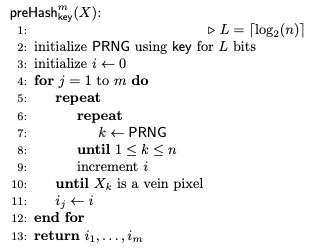
\includegraphics[width=0.5\linewidth]{latex-img/pseudocode_preHash.png}
    \caption{\textit{preHash} Algorithm}
    \label{preHash Algorithm}
\end{figure}

The algorithm, preHash, illustrated in Figure~\ref{preHash Algorithm} generates \(m\) smallest indices, denoted by \(i_j\), such that \(j\in{[1, m]} \) and \(1 <= i_1 < ... < i_m\), where each \(i_j\) correponds to an index such that \(X_{PRNG_{key}(i_j)} = 1\). It achieves this by rigorously verifying that the numbers produced by PRNG (PRNG[i]) stay within the specified bounds \(\text{PRNG}[i] \in (0, n] \text{ for } i \in [0, m]\).

\subsection{Assessing Similarity of Biometric Inputs After PreHash Application}

After the finger images are processed through the pipeline described in Pipeline~\ref{pipeline_simon} to extract their feature vectors, and the \textit{preHash} algorithm is applied, the outcome is a set of indices that fall within the inclusive range \(\text{PRNG}[i] \in (0, n] \text{ for } i \in [0, m]\), effectively mapping each selected feature to a unique index within the feature vector's length.

In the context of a simplified scenario where the hash length parameter (\(m\)) is set to \(1\), implying the generation of a single-index hash, and assuming a randomly chosen key for the \textit{preHash} algorithm, along with \(k\) representing a uniformly distributed random index, the probability that the \textit{preHash} operation yields the same index for two different inputs \(X\) and \(Y\) can be mathematically delineated as follows:

\begin{equation} \label{eq:preHash1}
    \begin{aligned}
        Pr[preHash_{key}^1(X) = preHash_{key}^1(Y)] &= \sum_{i > 0} Pr[preHash_{key}^1(X)]\\
        &= preHash_{key}^1(Y)\\
        &= \sum_{i > 0} Pr[X_k = Y_k = 0]^{i - 1} Pr[X_k = Y_k = 1]\\
        &= \frac{Pr[X_k = Y_k = 1]}{1 - Pr[X_k = Y_k = 0]}\\
        &= \frac{HW(X \land Y)}{HW(X) + HW(Y) - HW(X \land Y)}\\
        &= \frac{1}{\frac{1}{Score(X, Y)} - 1}
    \end{aligned}
\end{equation}

This equation encapsulates the likelihood of two images, \(X\) and \(Y\), having their singular hash index coincide, based on the presence of matching features identified by the algorithm. The final form of the equation relates the probability to the scoring function between \(X\) and \(Y\), inversely proportional to the score minus one.

It is noticed that there is a direct link with the Miura matching score that is of interest. The direct link between the \textit{preHash} algorithm's outcomes and the Miura matching score lies in their shared foundation of evaluating biometric similarities. Specifically, both methodologies utilize Hamming weight and bitwise operations to assess the overlap between biometric samples, such as finger vein patterns. The \textit{preHash} algorithm, through its probabilistic formula, quantifies the likelihood of matching indices based on feature presence, closely paralleling the Miura score's approach of comparing binary patterns to derive a similarity score. The above computation can also be expressed as follows:

\begin{equation} \label{eq:preHash2}
    \begin{aligned}
        Pr[preHash_{key}^1(\bar{X}) = preHash_{key}^1(\bar{Y})] &= \frac{Pr[\bar{X}_k = \bar{Y}_k = 1]}{1 - Pr[\bar{X}_k = \bar{Y}_k = 0]}\\
        &= \frac{\frac{Pr[X_k = 1] + Pr[Y_k = 1]}{2} - \frac{1}{2}Pr[\bar{X}_l \neq \bar{Y}_k]}{\frac{Pr[X_k = 1] + Pr[Y_k = 1]}{2} + \frac{1}{2}Pr[\bar{X}_l \neq \bar{Y}_k]}\\
    \end{aligned}
\end{equation}

The following approximations are made, inspired by equations p (\ref{eq:proba}) and $\delta$ (\ref{eq:delta}):

\begin{equation}
    E\left(\frac{\frac{Pr[X_k = 1] + Pr[Y_k = 1]}{2} - \frac{1}{2}Pr[\bar{X}_l \neq \bar{Y}_k]}{\frac{Pr[X_k = 1] + Pr[Y_k = 1]}{2} + \frac{1}{2}Pr[\bar{X}_l \neq \bar{Y}_k]}\right) \approx \frac{p - \frac{\delta}{2}}{p + \frac{\delta}{2}}
\end{equation}

The core of this approximation revolves around the expectation formula, which integrates probabilities of feature presence \(Pr[X_k=1]+Pr[Y_k=1]\) and the likelihood of discrepancies between \(X\) and \(Y\), \(Pr[\bar{X}_l \neq \bar{Y}_k]\). This formula essentially aims to quantify the similarity between two biometric samples by considering both the concurrence of features and the instances where they diverge.

Hence for (\(X\), \(Y\)) random,

\begin{equation}
    Pr[preHash_{key}^1(offset_X * X) = preHash_{key}^1(offset_Y * Y)] \leq \frac{p - \frac{\delta}{2}}{p + \frac{\delta}{2}}
\end{equation}

where equality is reached for the optimal offset translations. 

Depending on the distribution of (\(X\), \(Y\)), it is denoted

\begin{equation} \label{eq:mu}
    \mu = \frac{p - \frac{\delta}{2}}{p + \frac{\delta}{2}}
\end{equation}

The following figures are provided:

\begin{table}[H]
    \centering
    \renewcommand{\arraystretch}{1.25}\begin{tabular}{|c|c|c|}
        \hline
        $\mu_{same}$ & $\mu_{diff}$ & $\mu_{indep}$\\
        \hline
        $24\%$ & $8.3\%$ & $1.8\%$\\
        \hline
    \end{tabular}
\caption{Comparison of Distributions: $\delta_{same}$, $\delta_{diff}$, and $\delta_{indep}$}
\end{table}

Finally, it is observed that

\begin{equation}
    Pr[preHash_{key}^m(offset_X * X) = preHash_{key}^m(offset_Y * Y)] \leq \mu^m
\end{equation}

where equality is reached for the optimal offset translations.

%This includes determining the upper limits for the probabilities of similarity between different finger veins processed through the same fuzzy hashing parameters. 
\subsection{Experimental Derivation of the Probabilities \(\mu_{\text{same}}, \mu_{\text{diff}}, \mu_{\text{indep}}\)}

% Start this subsection by introducing the mathematical and theoretical concepts that underpin fuzzy hashing. Discuss the relevance of these concepts in the context of biometric data, focusing on how they enable the creation of reliable and secure hashing mechanisms for inherently noisy data.

%     Key Concepts to Cover:
%         Definition and significance of fuzzy hashing
%         Mathematical principles governing the construction of fuzzy hashes
%         Overview of the biometric setting, including the importance of parameters such as pixel dimensions, vein extraction, and the role of random permutations in hashing

% Subsection 2: Experimental Approach

% In the second subsection, outline the methodology of your experiments designed to test the theoretical underpinnings discussed earlier. Describe the setup, the specific objectives of each experiment, and how these experiments are structured to validate the theoretical models of fuzzy hashing.

%     Key Components to Include:
%         Description of the experimental setup and the data used
%         Explanation of how the experiments are designed to reflect the theoretical aspects of fuzzy hashing
%         Details on the implementation of preHash and postHash functions, and the criteria for their evaluation

% Subsection 3: Verifying Theoretical Predictions

% The final subsection is dedicated to comparing the outcomes of your experiments with the theoretical expectations. This involves analyzing the results, discussing any deviations or confirmations, and what these mean for the validity and reliability of fuzzy hashing in biometric data security.

%     Important Aspects to Discuss:
%         Analysis of experimental results against theoretical predictions
%         Discussion on the accuracy of the fuzzy hashing process, including the matching scores and error rates
%         Implications of the findings for biometric data security and future research directions

% Conclusion of Section 1

% Conclude with a summary of the insights gained from bridging theoretical concepts with empirical evidence. Highlight the importance of this integration for advancing the field of biometric security through fuzzy hashing. Reflect on the potential for future developments and applications stemming from your findings. --> Avons nous vraiment besoin de ça dans cette partie?